%\documentclass[12pt,preprint]{aastex}
\documentclass[12pt,preprint]{emulateapj}
\usepackage{graphicx}

\shorttitle{The PARAS Precision RV Spectrograph}
\shortauthors{Chakraborty et al.}
\slugcomment{Submitted for publication in PASP}
%\received{2010 July 1}

\begin{document}

\title{The Stabilized High Resolution PARAS Echelle Spectrograph: Instrument Description \& First Light Radial Velocity Results}

\author{
  Abhijit Chakraborty\altaffilmark{1},
  Suvrath Mahadevan\altaffilmark{2,3},
  Arpita Roy\altaffilmark{2,3},
  Eric Harvey Richardson\altaffilmark{4}
  F. M. Pathan\altaffilmark{1},
  Vishal Shah\altaffilmark{1},
  Rohit Deshpande\altaffilmark{2,3},
  Priyanka Chaturvedi\altaffilmark{1},
  Rajesh Shah\altaffilmark{1},
  V. Venkatramany\altaffilmark{5}
}
\email{abhijit@prl.res.in}
\altaffiltext{1}{Division of Astronomy ,
  Physical Research Laboratory, Navrangpura, Ahmedabad 380015, India}
\altaffiltext{2}{Department of Astronomy and Astrophysics,
  Pennsylvania State University, 525 Davey Laboratory, University
  Park, PA 16802}
\altaffiltext{3}{Center for Exoplanets \& Habitable Worlds,
  Pennsylvania State University, 525 Davey Laboratory, University
  Park, PA 16802}
\altaffiltext{5}{Aditya High Vaccum Private Limited, Ahmedabad- 280015, India}
%%%%%%%%%%%%%%%%%%%%%%%%%%%%%%%%%%%%%%%%%%%%%%%%%%%%%%%%%%%%%%%%%%%%
\begin{abstract}
We present here the instrument details and first-light precision radial velocity results from the PRL optical fiber-fed high
resolution cross-dispersed Echelle Spectrograph (PARAS) that has recently been commissioned at the Mt Abu 1.2m telescope. PARAS is capable of a single-shot spectral coverage of
3700  \AA\ to 8600  \AA\ at a resolution of $\sim60,000$. The spectrograph is maintained under stable conditions
of temperature, and enclosed in a vacuum vessel. The blaze peak efficiency of the spectrograph itself is  $\sim 30\%$ between 4500\AA\ and 6500\AA\ .  The stable PSF, wide wavelength coverage, environmental control, and use of a simultaneous calibration fiber enables PARAS to be used for a variety of exoplanets and stellar astrophysics projects.  The first-light radial velocity results show $2-3$ m/s over a period of 5 days using bright RV standard stars, even withougt the vacuum pulled. Such stabilized controlled instruments, even on moderate aperture telescopes, can contribute significantly to ongoing radial velocity searches for low-mass stars due the the large amount of observing time such dedicated facilities will be able to spend observing bright stars at a high cadence.
\end{abstract}

\keywords{planetary systems -- techniques: spectroscopy -- techniques:
  radial velocities -- stars: individual (47 UMa, $\sigma$ Dra)}

%%%%%%%%%%%%%%%%%%%%%%%%%%%%%%%%%%%%%%%%%%%%%%%%%%%%%%%%%%%%%%%%%%%%

\section{Introduction}
\label{introduction}
\indent The number of known exoplanets planets has growing rapidly in the last decade, with over 550
confirmed exoplanets known to date \footnote{see exoplanet.eu website}, with most of these confirmed
planets having been discovered using radial velocity technique. Small 1 to 2m aperture telescopes equipped
with highly stable fiber fed spectrographs are required for significant contributions since discovery and
characterization of exoplanet systems requires high precision radial velocity time-series spanning from weeks
to decades. The full characterization of many exoplanets may be achieved using such long time based observations.
Fundamental questions such as a) the range of planetary system architectures, and b) statistics of planets
in the habitable zone can be addressed once we began to observe host stars over very long period of time line.

The window for small telescopes relies in the fact a) a very large number of stars up to 12th magnitude
are yet to be monitored with high resolution spectroscopy for exoplanets studies, stellar seismology and
pulsations, and other related sciences like abundance measurements, stellar rotational velocities, and b)
a very large number of nights that are required for such science endeavors can only be available on 1 to 2m
class telescopes.

We at PRL have started our own exoplanet program using the technique of precision Doppler radial-velocity
measurements. For this we have designed and built an optical fiber fed high-resolution echelle spectrograph,
which is attached to our 1.2m Telescope at Mt. Abu, India. Here we report the spectrograph design in a pressure 
and temperature control environment,the first-light RV measurements and the stability of the spectrograph. 
PARAS stand for PRL Advanced Radial-velocity All-sky Search (see Chakraborty et al. 2008, 2010).


%%%%%%%%%%%%%%%%%%%%%%%%%%%%%%%%%%%%%%%%%%%%%%%%%%%%%%%%%%%%%%%%%%%%
\section{Motivation for a Highly Stablized  Spectroscopic Capability on the Mt Abu 1.2m Telescope}
\label{motivation}
\subsection{The Mt Abu 1.2 m Telescope}
The Mt. Abu telescope is located in the western part of India near the edge of the Thar desert at an altitude
of 1680 meters. The site enjoys good seeing conditions of median seeing of 1.3 arcsecs from October to February and 
about 1.8 arcsecs from March to June. Monsoon affects observations between July to mid-September. Typically we 
get about 220 cloud free nights in a year and out of which 150 nights may be photometric. The exoplanet project was
conceived at PRL with a aim to build a high resolution optical fiber-fed spectrograph under both temperature and
pressure controlled environment that will get about 80 to 100 nights in a year on the 1.2m Abu telescope. Our primary
motivation was to go for exoplanets around F/G/K stars and to obtain long term stability of sub-3m/s on bright stars
and 5 to 6m/s on fainter targets. 
\subsection{ The PARAS Project}
There is a clear scientific need for high-resolution spectrographs under temperature and pressure controlled environment 
that will give precise radial velocity measurements of stars (at 1 to 5 m/s precision) for various astrophysical studies 
like planet searches, stellar pulsations etc. Further, optical fiber-fed high resolution spectrographs on small telescopes 
using the simultaneous referencing technique have a clear advantage on radial-velocity (RV) precision sciences. Since
such spectrographs use the wavelength range from 4000\AA\ to 6800\AA\ for the radial velocity measurements, 
thus enhancing the Q factor and making it possible to achieve 5m/s precision on stars up to 10th magnitude 
using 1m class telescopes (Bouchy et al 2001, Queloz \& Mayor 2001, Queloz et al.2001). Recent success of such 
fiber-fed spectrometers coupled with small telescopes (1-2 m) proves the case. For example the Sophie 
spectrograph on the 1.9m telescope in France (Bouchy et al. 2006, 2010) and the CORALIE spectrograph (Queloz et al. 2000). 
The CORALIE on a 1.2m telescope has been involved in the detection or confirmation of 54 extra-solar planet candidates, 
with RV precision of 5 to 6m/s at S/N ~ 50 on stars up to 10th magnitudes in reasonable exposure times 
(Segransan et al. 2009).   

%%%%%%%%%%%%%%%%%%%%%%%%%%%%%%%%%%%%%%%%%%%%%%%%%%%%%%%%%%%%%%%%%%%%
\section{Comparision with other optical precision RV spectrographs}
%%%%%%%%%%%%%%%%%%%%%%%%%%%%%%%%%%%%%%%%%%%%%%%%%%%%%%%%%%%%%%%%%%%%
\section{PARAS: Optical Design \& Components}
\label{optdesign}
Blah Blah Blah top level, white pupil design blah blah blah. Optical design Figure. Point to Appendix for a Zemax file description.

The spectrograph is designed with an aim of extreme stability for doing precision radial velocity measurements
down to a few meter/sec (<3m/s) with a basic spectrograph resolution of R~60000 between 3700A to 8600A. Its an
optical fiber fed R3.73 (blaze angle of 75 ; made from Master MR160 from Richardson Gratings) Echelle white pupil
spectrograph with a single prism as a cross disperser and three elements one singlet, one triplet and one doublet
Camera lens system. Since the spectrograph is planned for a small telescope of 1.2m aperture care has been taken
for minimal light loss in the optics train and the detector quantum efficiency. Details of the design
considerations are given in Chakraborty et al. (2008), however, we have made some changes in the glasses of the
Camera system for higher throughput in the blue wavelengths and also the logistics of practical availability of
large amount of glass. The Glass PKZ52 Scott glass has been changed to S-FPL52Y Ohara glass. The spot sizes
remained unchanged.

\subsection{Fiber Feed, Input optics, and scrambler}
We are using Multi-mode fiber, FBP type, core 50microns, including clad ~85microns, 20m in length, very good
transmission over 20m length, only up to 15\% light loss due to the length of the Fiber. The Star fiber and the
Calibration fiber form a bundle on the spectrograph side such that these two fiber cores are separated by
180microns +/- 3microns which corresponds to about 17 pixels separation of the spectra on the Detector.

On the spectrograph side F/4 beam coming out of the fiber tips are first collimated by a F/4 doublet and
re-imaged on to the slit position using a F/13 Doublet; both the doublets are custom made achromats defining
spot sizes within 20microns diameter; the Calibration fiber has the same configuration of Lenses at the other end
Projected 50micron fiber diameter at the slit position and resolution R ~170microns corresponding to
Resolution (R) ~63000; there is no slit at the slit position. The projected fiber image defines the resolution,
thus avoiding slit losses.

One of the primary issues we are encountering while coupling the fiber optics with the telescope is
that of the telescope flexure between the Primary mirror and the secondary mirror and also the telescope
tracking error. Since the telescope runs on an old technology, it has tracking accuracies of only 2arcsecs
and suffers from hysteresis in RA and DEC drives and also huge flexures and hence alignment issues between
the primary and the secondary. Thus, due to flexure alone, the star image moves in the focal plane by several
hundreds of microns as it tracks the star from East to the West. Therefore, we introduce the star-light into the
the star fiber in the following manner: the 1.2m telescope F/13 beam is converted into F/4.5 using a Focal reducer 
and the 50micron star fiber tip directly inserted in the F/4.5 telescope focal plane, the fiber see about 2-arcsec on the sky;
We have built a special instrument with precision actuators (from Physik Instruments) that can move the fiber tip in the telescope focal plane with a precision of 3microns. This system is guided by a Guide CCD which gathers only 8\% of unfiltered light using 
a pellicle beam splitter just above the telescope focal plane but after the focal reducer in the F/4.5 beam. 
The X-Y actuators moves the fiber tip and centroid on the star, and guides on the star with an accuracy of 1 to 1.3 arcsecs.
This instrument enables us to take exposure times of several 10s of minutes without the losing the star from the 
Fiber-tip at the telescope focal plane.
\subsection{OAP Collimators}
Off-axis parabolic mirrors M1 \& M2 Zerodur Glass, Cut from 60cm diameter Parabola, M1 is 140.5mm x 260.5mm x (54mm, thickness), Off-axis 127.5mm +/-0.5mm, Radius 2595mm +/-0.6mm; M2 is 130.5mm x 260.3mm x (55.5mm thickness), Off-axis 158.5mm +/-0.5mm, Radius 2595mm +/-0.6mm;
Surface quality of M1 and M2 are: Surface Front Error (SFE) within the useful area ~11nm(M1), 18nm(M2) rms, Periodic errors are at ~2.5nm, Micro Surface Roughness at ~1.5nm; Reflectivity (R): Special Protective Silver Coating, 4000A to 9000A > 95.5\% (98.5\% max at 7500A), 3800A to 4000A > 92\%; Manufactured and Coated by SESO
Flat Fold mirror (FM)   Zerodur Glass, 160.44mm x 16.44mm x (33mm, thickness), SFE in the useful area ~ 19nm, Periodic errors ~ 1.5nm, Micro Surface Roughness < 1nm; Reflectivity: Same as M1 \& M2 mirrors; Manufactured \& Coated by SESO.
\subsection{Grating}
Echelle Grating Dimension of 420.5mm x 220.5mm x 74mm; Useful ruled area 415mm x 215mm, Blaze angle 75 , used in Littrow condition, face down, with a small   angle of 0.45 ;
Surface quality  $\lambda$/4 P-V over the central region and almost 70\% of the ruled area, this region is used by the 100mm diameter pupil, thus ensuring a higher spectral purity; Blaze peak up to 63\% efficient for each order; Manufactured by New-Port Richardson Gratings
\subsection{Prism}
Prism   OHARA, PBM8Y glass, apex angle 65.6 , physical size of entrance and exit faces are about 226mm x 170mm; Prism Height 190.8mm; Transmitted Wave-front Error ~ 72nm rms; Surface roughness within the useful area ~1.5nm; Throughput efficiency measured at ~81\% between 3800A and 8500A including both surfaces; Cut, polished and AR-coated by SESO
\subsection{Camera}
Camera Lens System  F/5, Focal Length ~528.5mm at 6330A, EE80 (diameter) on-axis and at +/-3.1  field ~ 9microns, 96\% of encircled energy with in 25microns; Average transmission thru the Lens system (total six surfaces) ~ 95\% between 4000A and 8600A; Manufactured, assembled and Zygo Interferometer test is done by SESO
\subsection{CCD}
To enable efficient coverage of the broad bandwidth of the PARAS spectrograph we selected the 4096x4096 E2V CCD231-84-1-D81 device as the detector array. This CCD has 15 $\mu m$ square pixels, is a deep depletion device, and has a custom E2V "astro-broadband" anti-reflection (AR) coating that provides high quantum efficiency (QE) over most of the operating wavelength of PARAS.  While a graded AR coating, to maximize efficiency, would have been possible \citep{Kelt06, Raskin11}, the deep depletion device does not exhibit any significant fringing at red wavelengths, making the standard coating sufficient for our purposes. Table \ref{table:QE} shows the measured QE for the PARAS science array at specific wavelengths.

\begin{table}[h]
\begin{center}
\label{table:QE}
\caption{Measured Quantum Efficiency of the PARAS Science CCD Array}
\begin{tabular}{ c | c }
 \hline
  Wavelength (nm) & Quantum Efficiency (QE)  \\
  \hline
  350 & 57.2\%  \\
  400 & 92.4\%  \\
  500 & 96.5\%  \\
  650 & 87.9\%  \\   
  900 & 51.9\%  \\     
  \hline  
\end{tabular}
\end{center}
\end{table}

The CCD Dewar and cryogenic assembly was built by Infrared Laboratories. To minimize vibrations caused by the closed cycle cooling we employ a low vibration Cryo-Cooler DMX-20 head  from Advanced Research Systems Inc. that uses a Helium closed cooling system to achieve cooling as well as a vibration amplitude of $< 150 nm$ at the detector plane. The used of this closed cycles system eliminates the possibility of slow velocity drifts due to changing moment of inertia if a liquid nitrogen system were to be used.  A Lakeshore model 331 temperature controller is used to maintain the CCD at its optimum operating temperature of -120 C. CCD control and data acquisition are accomplished with a SDSU Gen-III controller and associated electronics.  A computer ruling Red-Had Linux is used to acquire and display the data. The CCD exhibits a dark noise of $\sim 0.02$ electrons/pixel/hour at the standard operating temperature, and the slow-readout mode with the controller yields a read noise as low as 3.5 electrons.

%%%%%%%%%%%%%%%%%%%%%%%%%%%%%%%%%%%%%%%%%%%%%%%%%%%%%%%%%%%%%%%%%%%%
\section{Mechanical Design \& Vaccum Enclosure}
The Vacuum Chamber is made of Stainless Steel 304L material and has large rectangular port openings for easy access to optical components placed inside the chamber.  The ports are covered using flanges made of Aluminum.  Both the materials are vacuum compatible and can hold vacuum with vacuum pumps isolated, due to low out-gassing properties. The shape of the vacuum chamber was optimally chosen to enclose the entire optical path from the slit position to the CCD Dewar.  Thus one axis of the chamber is about 2 m in length while the other is about 1.6 m.  The height of the vacuum chamber is about 0.7 m and is designed to enclose partly the CCD dewar, leaving the Helium line connections for cryo-cooling outside the vacuum chamber. This arrangement is done through flexible stainless steel bellows.  The base plate of the vacuum chamber acts as the optical bench and has a surface flatness of 20 microns.  The optical axis is 300 mm above the optical bench.

The base plate and the port flanges are adequately strengthened by external ribs, and the chamber walls are strengthened by internal ribs to give minimum deformation under vacuum.  ANSYS CAE (Computer Aided Engineering) Software Program was used in conjunction with 3D CAD (Computer Aided Design) solid geometry to simulate the behavior of mechanical bodies under thermal and structural loading conditions.  ANSYS automated FEA (Finite Element Analysis) technology was used to generate the results. The analysis was done for static structural deformation and stress at three uniform ambient temperature 0 C, 20 C, and 40 C for an external pressure of 1 atmosphere. The maximum deformation was ensured to be within 50 microns and maximum stress was ensured to be well within the minimum yield strength. Aditya High Vacuum manufactured the Chamber.

The evacuation of the Chamber is done using a Dry Vacuum Pump (Alcatel make, Multi-roots type) to a vacuum less than 10-1 to 10-2 mbar.  The vacuum is measured using an absolute pressure measurement gauge using capacitance manometer principle.  Liquid Nitrogen cooled Activated Alumina Trap improves the vacuum to the range of 10-2 to 10-3 mbar and also allows to hold the vacuum in the chamber at a steady value even after isolation of the Displacement pump.  The fabrication of the vacuum chamber is completed and tested for holding the vacuum at 10-2 mbar for over 36 hours. We have also tested the actual deformations and verified them against the theoretical ANSYS results, and they are as per expectation within 30microns and are well within the limits. We have also tested that as long as the holds the vacuum of 10e2 mbar the deformations remains constant for the stability of the spectrograph. (more to be written here on the Vacuum chamber)

The star fiber and the calibration fiber are taken into the vacuum chamber thru a special fiber feed-through, where the fiber teflon sleeve is symmetrically compressed to a diameter of 90 microns that is just barely touching the fiber. The Helium leak test of the connectors prove that the leak rate is of the order of 10e-8 through the teflon sleeve. The electrical connections are taken into the vacuum chamber through vacuum compatible multi-pin feed-throughs.

The spectrograph is installed in a closed concentric volume space consisting of the outer and the inner chambers. The optical bench is kept on vibration isolation RCC pillared (isolated from the observatory building by a few cm gap from all sides) polished Granite top table. The inner chamber is built around this special table. The walls of the chambers are made up of highly insulated 60mm thick puff material (materials similar to those used in standard commercially available refrigeration systems). The outer chamber temperature control is achieved at 20 C +/-0.8 C using standard Heating and Cooling mechanisms, which are commercially available. It is PID controlled and the temperature can be set at any value between 18 C and 24 C. We have tested it at 21 C and at 24 C with a precision of +/-0.8 C.

The inner Chamber has an inbuilt temperature control system. We control the temperature by increasing it about 2 C above the outer chamber temperature. Electronic Thermal controlling is used to control the heaters and record the data. We have used Pt100 temperature sensor, which is well known for its high stability, ~ 0.005\% or better than that. Pt100 along with associated pre-amplifier convert the temperature into equivalent analogue values. The ADC (ADC7135) converts this analog information from the sensor to digital information with a resolution of 0.01 C. In the near future we plan to increase this resolution to 0.001 C. ADC reference voltage is highly stable. We have used REF200 from Burr-Brown. The sampling frequency is around 100khz. ADC output is compatible and connected with one of the port of microcontroller. We have used Atmel 89c51/52 microcontroller to digitize the temperature information and sending appropriate data to control the heater. A preset temperature value is required to enter to the microcontroller. The microcontroller compares this preset value with the current temperature. If there is a difference then it passes the appropriate digital value to heater circuitry and to heater power driver. The program is written in assembly language to display the temperature on LCD, and also simultaneously it also sends the temperature data Serially to PC through Comport (RS232). Data Acquisition Software is written in VISUAL BASIC to acquire the data and storing it in hard disk. (more to be written here)
%%%%%%%%%%%%%%%%%%%%%%%%%%%%%%%%%%%%%%%%%%%%%%%%%%%%%%%%%%%%%%%%%%%%
\section{Environmental Control: Temperature \& Pressure}
\subsection{Temperature Control \& Performance}
\subsection{Vacuum Chamber Stability \& Performance}
%%%%%%%%%%%%%%%%%%%%%%%%%%%%%%%%%%%%%%%%%%%%%%%%%%%%%%%%%%%%%%%%%%%%
\section{Spectral Format, Simultaneous Wavelength Covergage, \& Resolution}

\begin{figure}[htbp] %  figure placement: here, top, bottom, or page
   \centering
   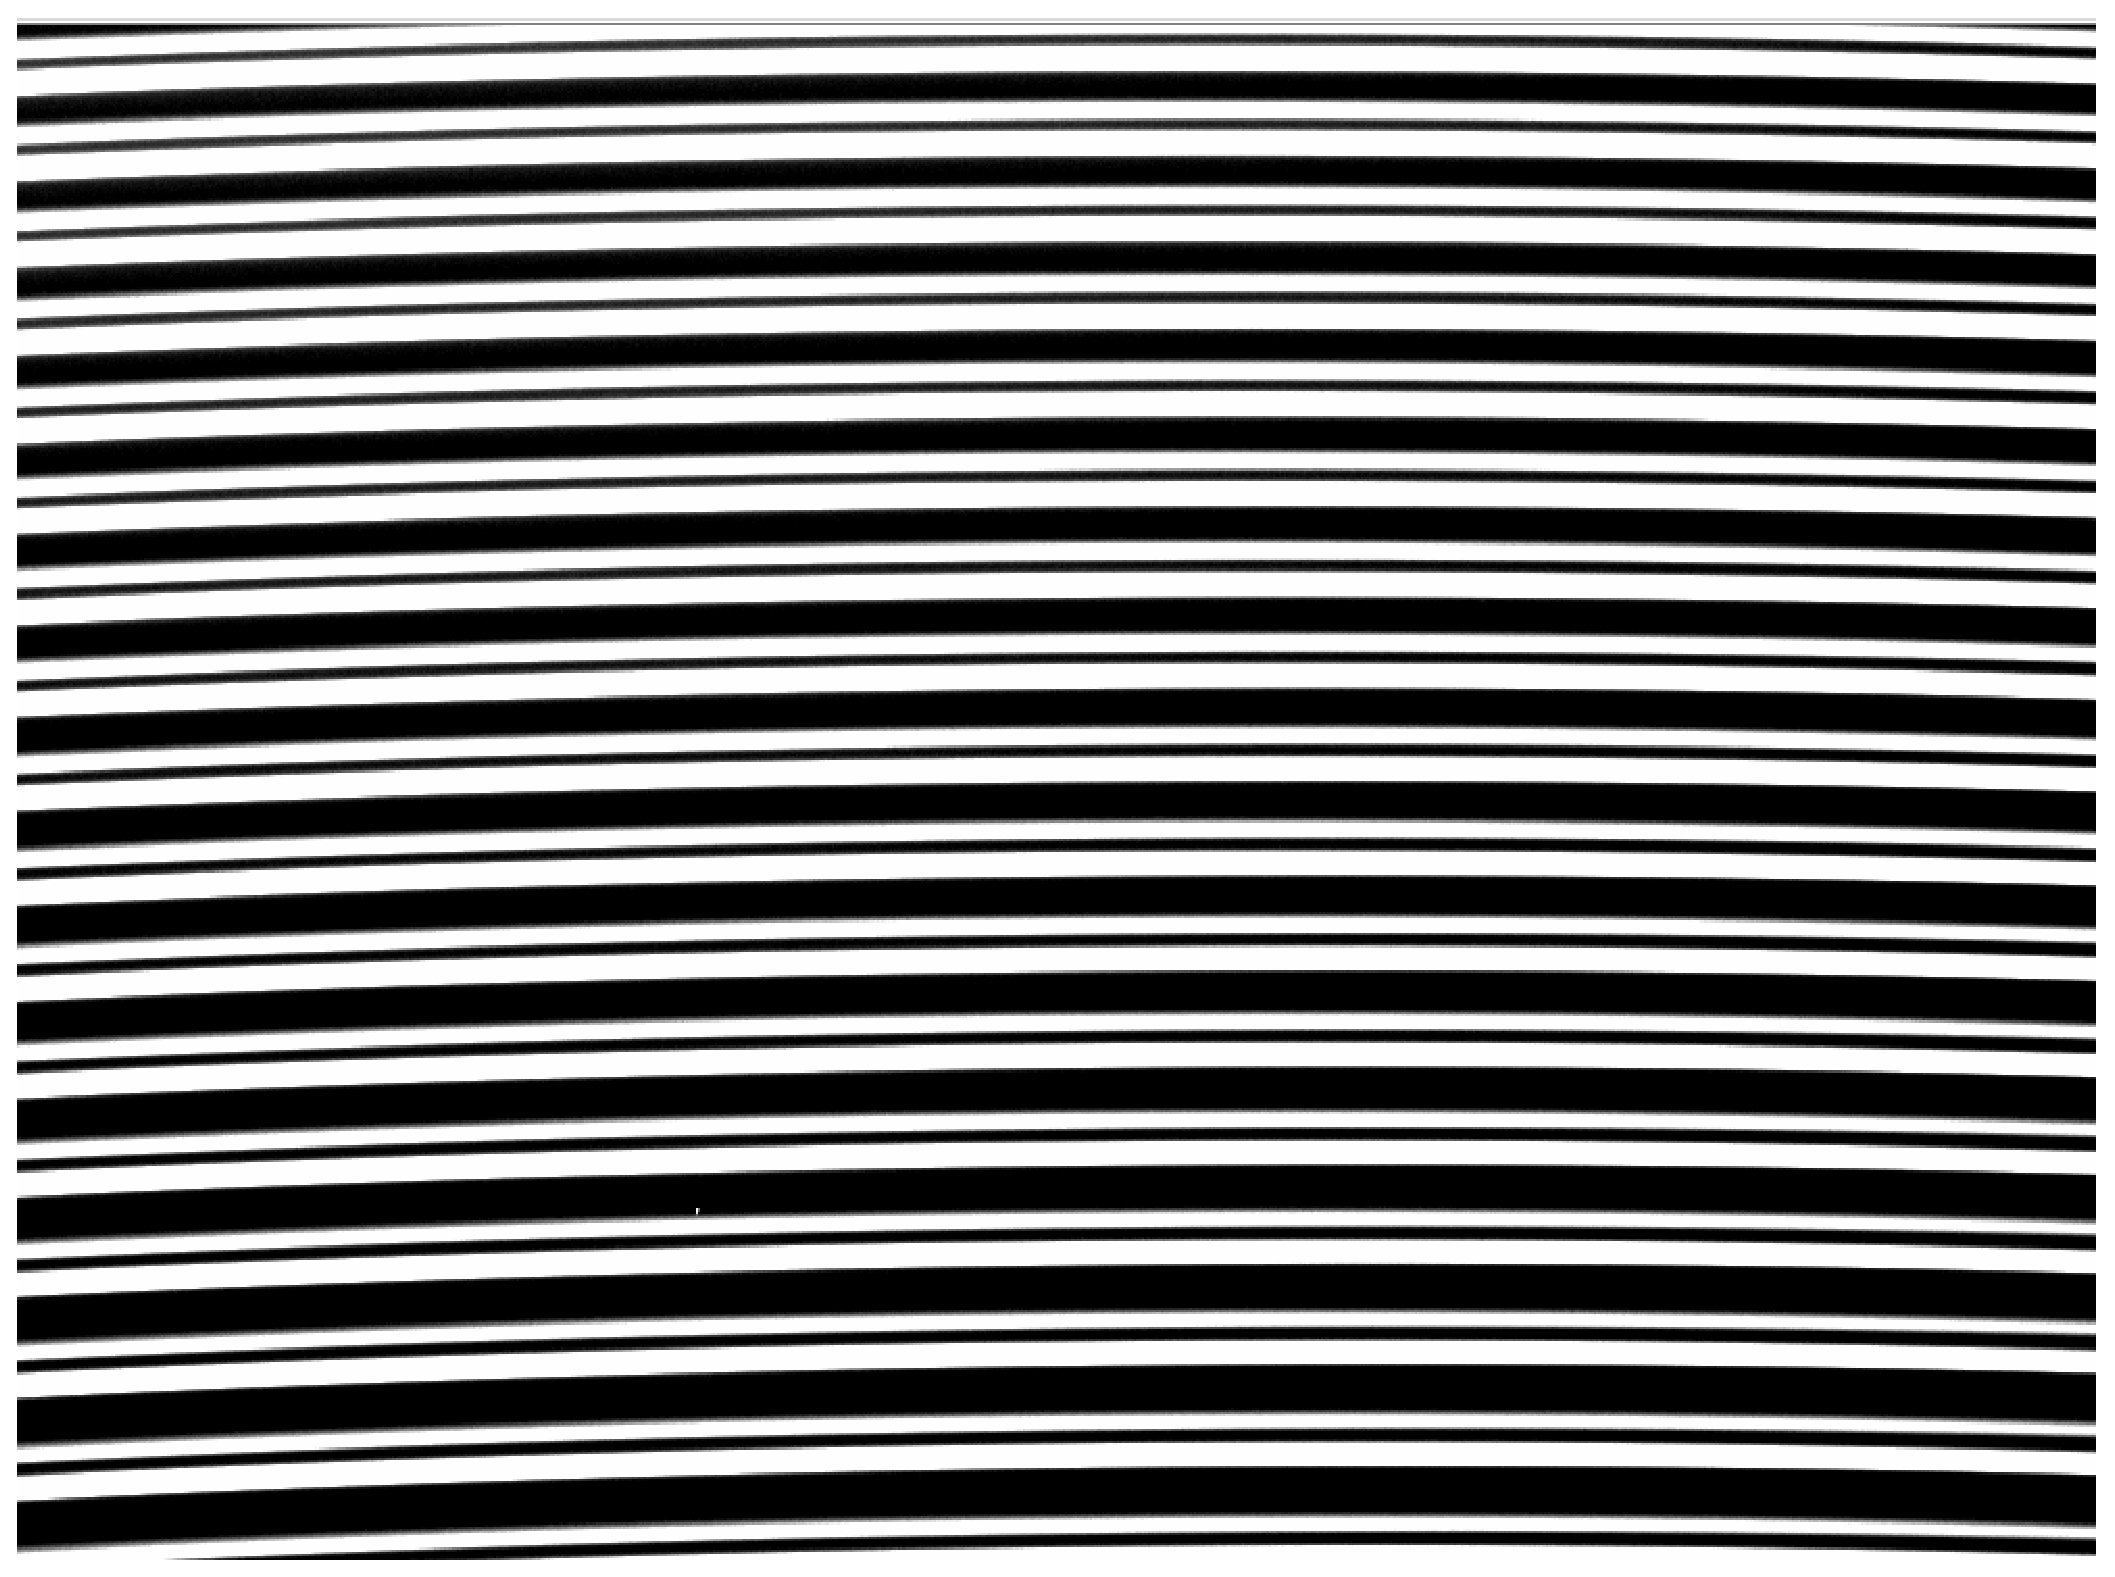
\includegraphics[width=0.21\textwidth, angle=90]{flat.eps} 
   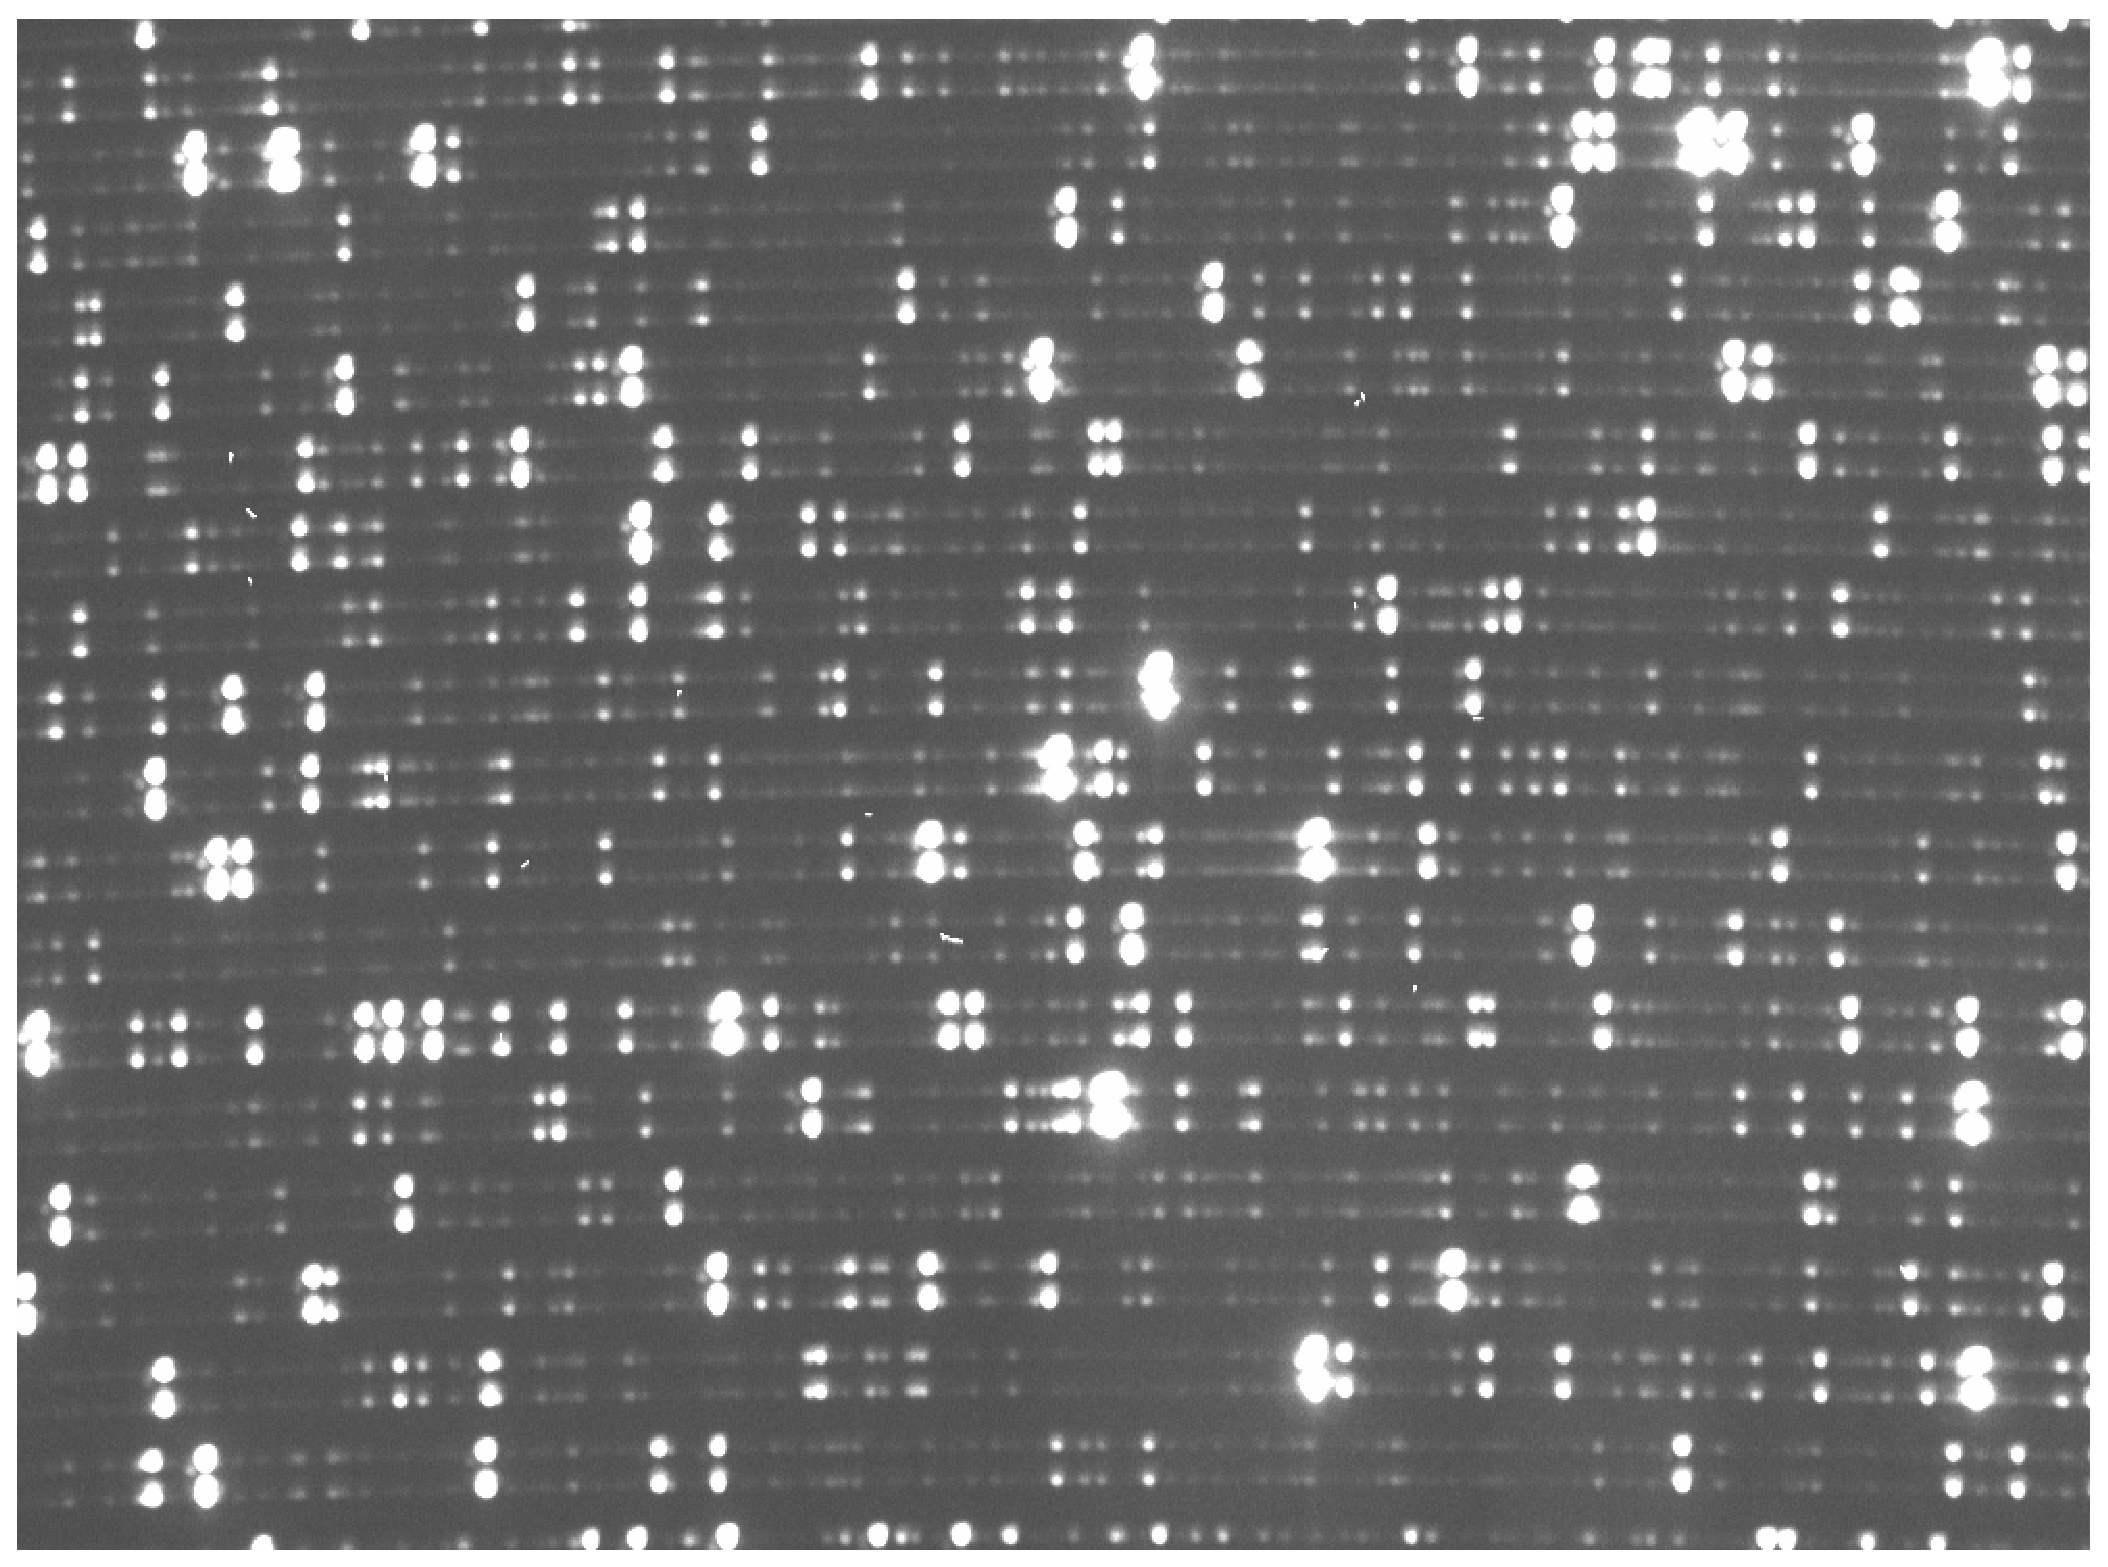
\includegraphics[width=0.21\textwidth, angle=90]{thar-thar2.eps} 
   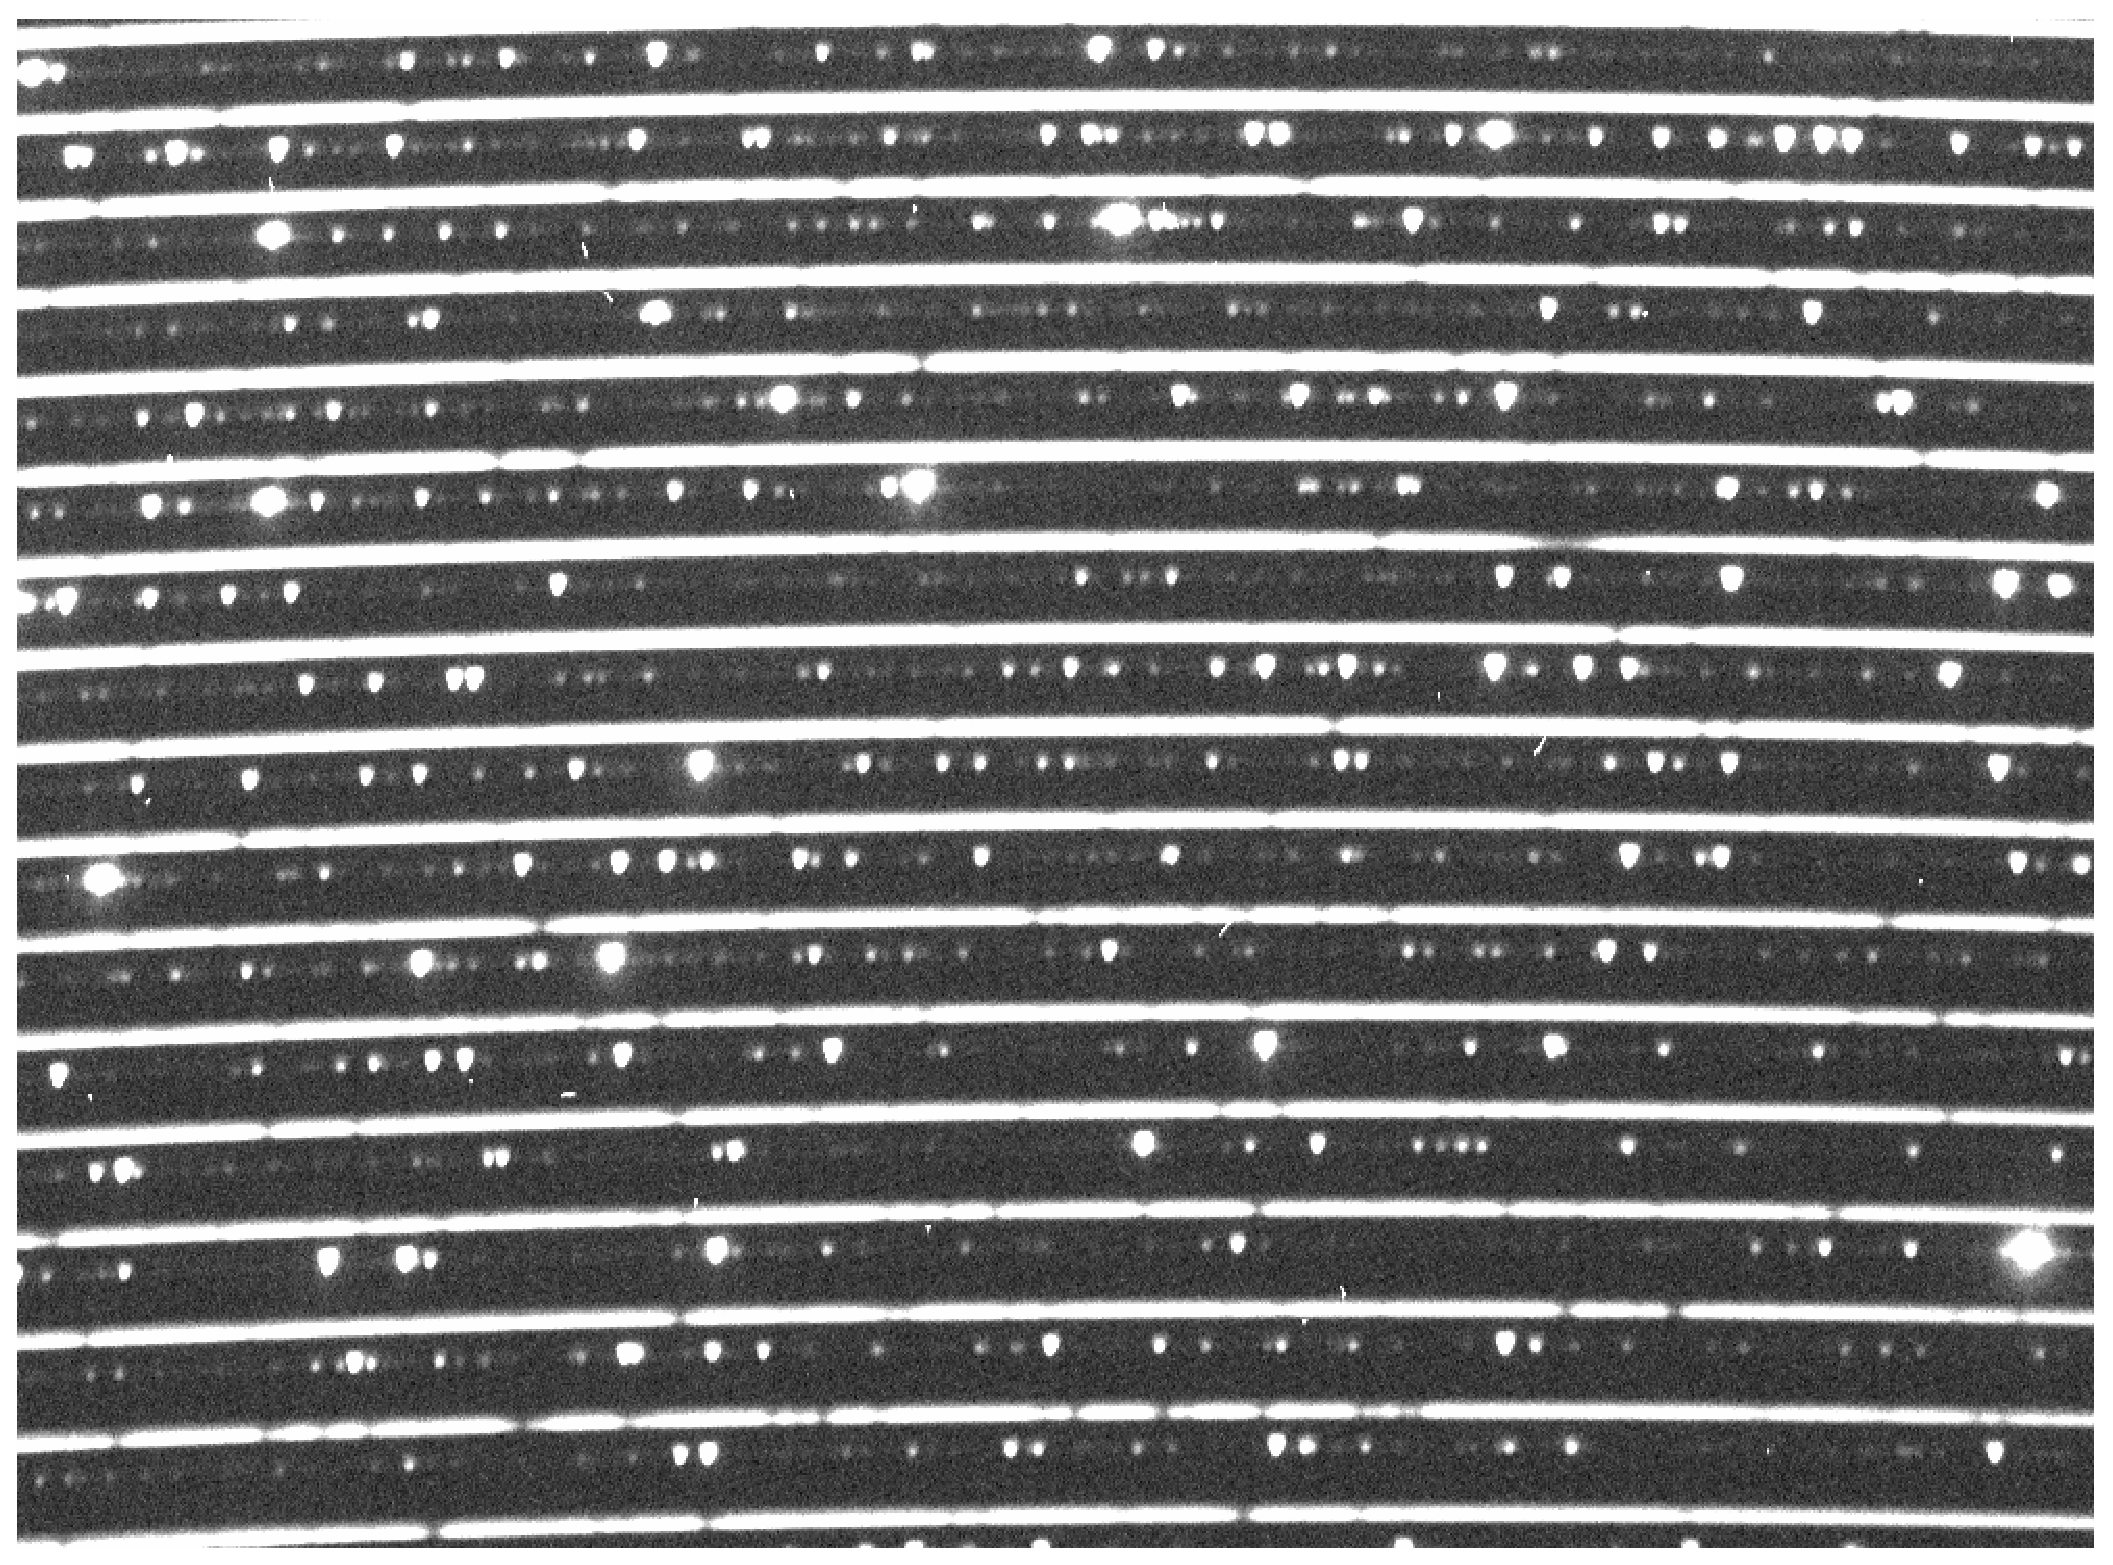
\includegraphics[width=0.21\textwidth, angle=90]{star-thar.eps} 
    \caption{Portion of raw image for {\bf (a)} flat field exposure, {\bf (b)} 
    thorium-thorium exposure, and {\bf (c)} stellar exposure with simultaneous
    thorium calibration.}
   \label{fig:frames}
\end{figure}

\begin{figure}[htbp] %  figure placement: here, top, bottom, or page
   \centering
      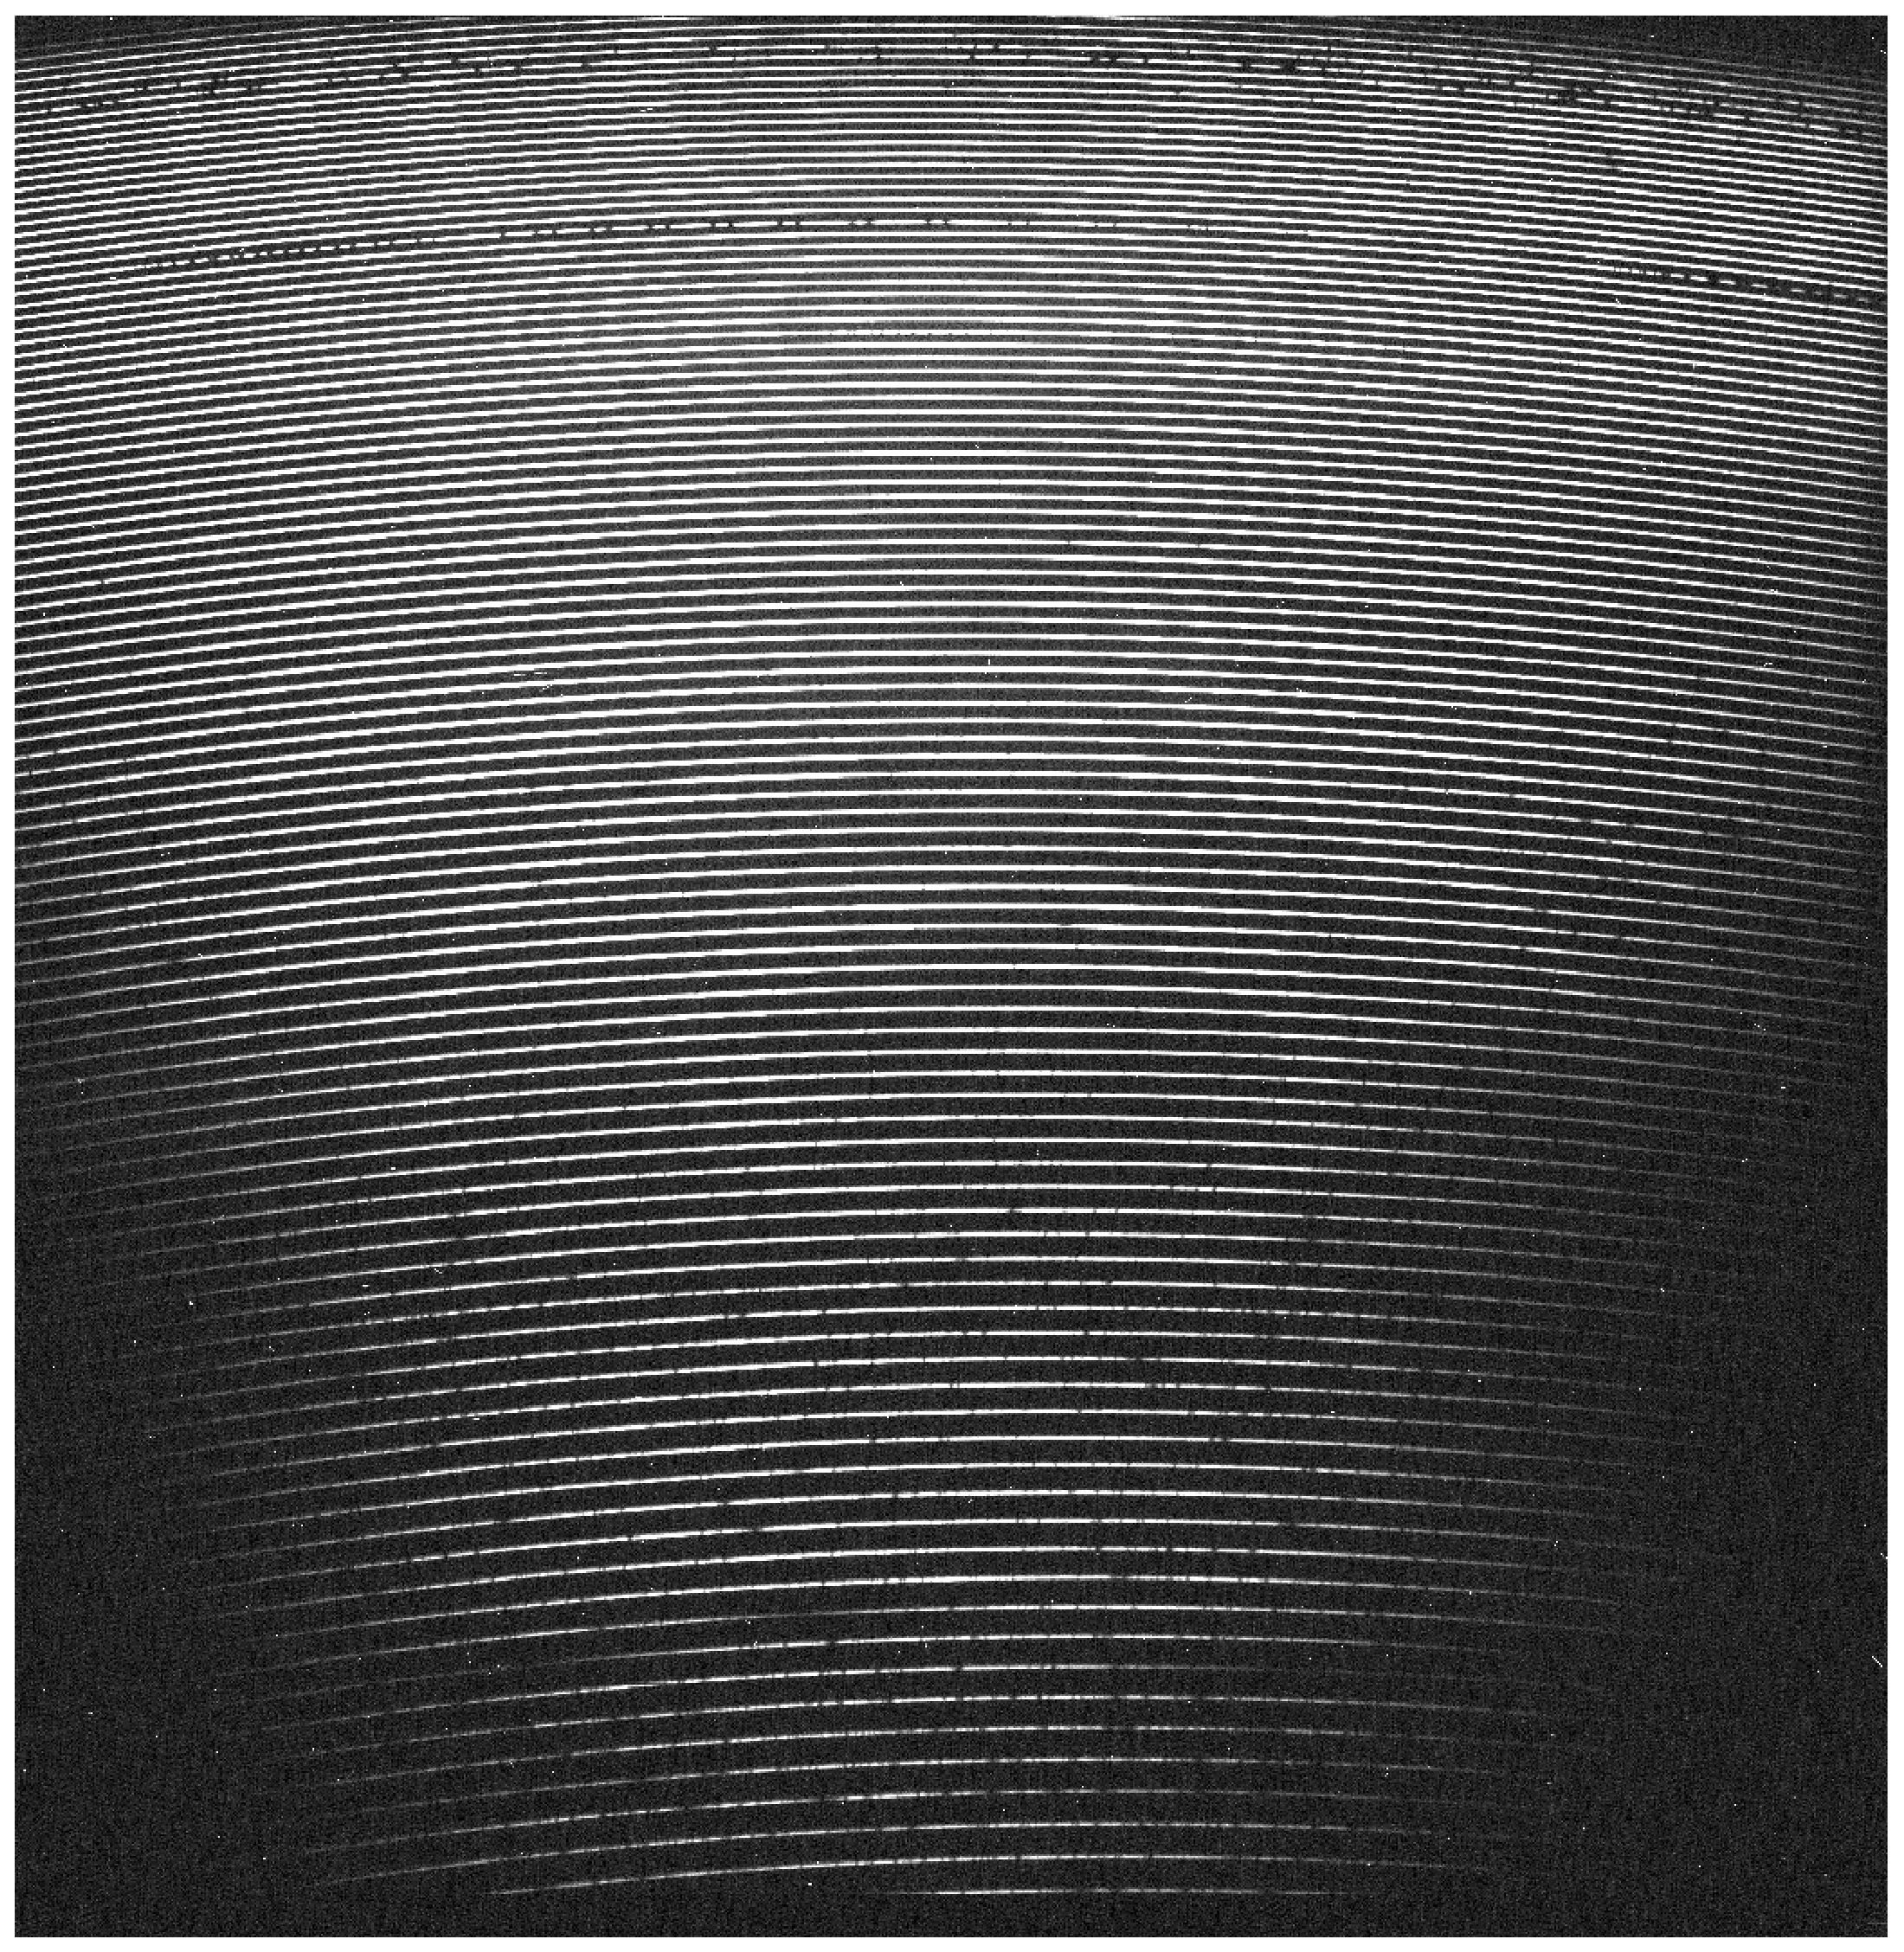
\includegraphics[width=0.5\textwidth]{full_star.eps}
    \caption{Full-frame raw image of a star (47 UMa), with single fiber illumination.}
    \vspace{10pt}
   \label{fig:fullstar}
\end{figure}

\begin{figure}[htbp] %  figure placement: here, top, bottom, or page
   \centering
   \includegraphics[width=0.5\textwidth]{3stars_paper_1_47uma_sigdra_hd137759.eps} 
   \includegraphics[width=0.5\textwidth]{3stars_paper_2_47uma_sigdra_hd137759.eps} 
    \caption{Illustrative section of extracted spectra. The stars shown are 47 UMa (G1V, black),
     Sig Dra (K0V, red), and HD137759 (K2III, blue).}
   \label{fig:3stars}
\end{figure}

\begin{figure}[htbp] %  figure placement: here, top, bottom, or page
   \centering
   \includegraphics[width=0.5\textwidth]{resolution_paper.eps} 
      \vspace{10pt}
       \caption{Measured spectral resolution of PARAS. The x-axis is in pixels and represents the actual
    CCD scale; the left y-axis is in orders and represents the portion of the chip underlying extracted spectra. 
    For illustrative purposes, the orders are shown only in one dimension (removing echelle order curvature). 
    Although the orders are shown evenly spaced, the wavelength axis on the right reflects the increasing
    proximity of redder orders. Notice that the top left of the image indicates some focussing issues, and that the
    lower corners have no useable lines because of low flux.
    }

   \label{fig:res}
\end{figure}

%%%%%%%%%%%%%%%%%%%%%%%%%%%%%%%%%%%%%%%%%%%%%%%%%%%%%%%%%%%%%%%%%%%%
\section{Cassegrain Feed and Calibration Unit}
%%%%%%%%%%%%%%%%%%%%%%%%%%%%%%%%%%%%%%%%%%%%%%%%%%%%%%%%%%%%%%%%%%%%
\section{Efficiency}

Specifically, Figure \ref{fig:efficiency} shows black body at 3200K * fiber transmission*mirror1*mirror2*mirror2(flat fold mirror)*camera*dewar window surface1*dewar window surface2*ccd*0.62 (ccd qe)

\begin{figure}[htbp] %  figure placement: here, top, bottom, or page
   \centering
   \includegraphics[width=0.5\textwidth]{efficiency_paper.eps} 
    \caption{Efficiency of the PARAS spectrograph, including fibers and detector. The dashed line shows calculated 
    efficiency and the solid line shows measured values. }
   \label{fig:efficiency}
\end{figure}

%%%%%%%%%%%%%%%%%%%%%%%%%%%%%%%%%%%%%%%%%%%%%%%%%%%%%%%%%%%%%%%%%%%%
\section{Data Analysis Pipeline}

\subsection{Reduction Pipeline}
The data reduction pipeline, written in the Interactive Data Language (IDL), is a fully automated, minimally subjective, highly reproducible, and robust set of image processing algorithms that allows batch-processing of large amounts of data. It requires user initiation but not interaction, unless troubleshooting becomes necessary due unexpected external factors. At the core of the pipeline is the REDUCE data analysis package for conventional and cross-dispersed echelle spectra developed by Piskunov \& Valenti (2002), which was adapted and evolved to meet the specific needs of the PARAS spectrograph. 

The pipeline uses sorted raw calibration and science data in FITS format to produce optimally extracted spectra of science targets. Composite calibration frames are created initially for each night. A master bias is made by co-adding all nightly bias frames in two groups and then combining them after a comparison for bias shifts, read noise effects, and outliers. This master bias frame is subsequently subtracted from all non-bias images. A master flat is similarly created by co-adding all available flats. Echelle order curvature and locations are determined empirically from a high quality flat field image in order to extract spectra with negligible continuum. REDUCE employs a two-dimensional clustering algorithm for this purpose, which selects potential spectral order pixels and tests the level of clustering before merging and rejecting partial orders, ultimately fitting the merged clusters. Since we have a large number of spectral orders, we enhance the performance of this routine by using a special mask that shrouds low signal corners of the image in addition to defining bad pixels. The order tracing routine requires user interaction for clusters that are not obviously meant to be merged or rejected. Therefore to automate the pipeline under the valid assumption that PARAS is a very stable instrument, in lieu of this interactive step we have a master order trace available that is employed whenever pixel shifts between nights are negligible. 

REDUCE uses a sophisticated decomposition routine to normalize flat field images, obtain order shape functions, estimate scattered light in inter-order gaps, and extract spectral orders. This involves a division of the image into swaths, whereby the spectrum (illumination profile along the order) is separated from the spatial profile for each column (relative illumination pro�le perpendicular to echelle dispersion). Starting with an initial guess for the spectrum, the spatial profile is fit using an empirically determined mean spatial profile, with weights based on a noise model. Iteration ceases when the change in the deduced spectrum becomes small, producing the best possible slit function and spectrum, under the assumption that the large scale structure in the image is spectral and that the order trace is valid. A major advantage of this method is that by assuming a smooth profile within an image swath, the influence of cosmic rays, bad pixels, and noise is minimized. We further assist the routine by providing known CCD defects in a bad pixel map.   

It is necessary to estimate the scattered light background for subtraction from both normalized flat field images and spectra, although the background beneath an order cannot be directly measured. Instead, an interpolation of the background between orders after the isolation of inter-order noise with the decomposition method, provides a good estimate. Sky emission is included in this estimate but the routine is not equipped to handle ghosts or very bright emission lines. The careful instrument design of PARAS ensures that scattered light removal has a minimal effect and that ghosts are not a major concern, but with a thorium-argon calibration source, bright argon lines in the redder parts are unavoidable. Although PARAS has a filter that sharply depletes light of wavelengths greater than 700nm, beyond which lies the brightest contamination, we find that with a prism cross-disperser, the high mutual proximity of the redder orders requires that the bleeding of bright argon lines into star orders be cured diligently. Even a simple linear column-by-column interpolation routine for scattered light subtraction improves pipeline performance in places where bright argon lines are incompletely removed; but our preferred method is to use a bleeding map, linearly scaled by global parameter describing variations in lamp brightness (similar to Lovis et al. 2011).

Flat fielding is necessary to remove pixel-to-pixel quantum efficiency variations, but the master flat must first be  normalized in order to minimize noise contributions and avoid magnifying low-signal regions of the image. Especially for a fiber-fed spectrograph like PARAS, where the flat field images have a spatial profile very similar to science exposures, regions at all signal levels must be carefully weighted. Inter-order regions are set to unity, and the order is divided into swaths before decomposition. The spectral profiles are spliced together to form the shape or blaze function for each order, while the spatial profiles for adjacent swaths are interpolated or extrapolated and subsequently scaled by the blaze to normalize each column segment in the master flat. Care is taken to choose the number of swaths so the the spatial profile is oversampled, while keeping the swath width large enough that changes in the point-spread-function along a spectral order can be tracked.      

Finally, REDUCE optimally extracts spectra using the same swath-based decomposition method described above. The science image is bias subtracted, divided by the normalized flat-field image, decomposed for scattered light correction, and decomposed again for optimized spectral extraction. Continuum normalization is achieved by dividing out the order shape function previously determined.

\subsection{Analysis Pipeline}

The spectra in pixel-order space must be wavelength calibrated using a template of suitable thorium lines. To create an approximate solution for the new instrument, a cursory line identification was initially performed to predict a two-dimensional wavelength function across the chip. This must be repeated every time the instrument is moved, or the order inclusion and locations change. However, with a stabilized instrument it is possible to have a blueprint wavelength solution of the simultaneous thorium-argon lamp spectra available to calibrate new data. Pixel shifts are cross-correlated out and missing orders noted; subsequently, the redetermination of emission line centers as indicated by a gaussian fit mutually produce polynomial coefficients to precisely define the graduation of wavelength across the order. A complete thorium line list for the PARAS spectral range is utilized (a combination of the SOPHIE, HARPS, and UVES atlases - cite?). A deviation threshold removes outliers and prevents noise from being mistaken as emission lines. The user can change both the level of error acceptable and the minimum number of lines used to define an order. 

In order to track instrument stability, we create a binary mask of reliable sharp thorium lines and use this in conjunction with periodic calibration lamp exposures throughout the night. The cross correlation function (CCF) is calculated for a shifting thorium mask against each spectral order, and the CCFs are summed in order to fit a gaussian peak to the true drift value of the image. For simultaneous thorium exposures on stellar spectra, this also yields the temporal instrument drift correction (Fig.\ref{fig:drift}). 

Radial velocities (RVs) are derived by cross correlating target spectra with a suitable numerical stellar template mask based on spectral type (with default G2), created purposely from high signal-to-noise or synthetic data (Baranne 1996). Mask lines are centered around bright absorption peaks, with a width of 3~km~s$^{-1}$ and a depth set by the star. On testing the effect of using all available mask lines, as opposed to only lines deeper than some threshold value, we find that using more lines leads to better RVs as expected, but also that there is a noise floor of about 2~m~s$^{-1}$ reached with lines deeper than 40\%, beyond which the inclusion of shallow mask lines has little effect -- possibly an instrumental artifact (Fig.\ref{fig:maskcut}).

We begin the algorithm for precision RVs by providing an estimate for the radial velocity of the star, to which the barycentric correction is applied. This centers the region of scrutiny, the range of which is used to recreate the mask at regular intervals to produce a CCF for each order. The maximum number of useable order CCFs (with no saturated regions) are then summed and fit to obtain the radial velocity of the observation. Instead of using the wavelength calibration of each simultaneous thorium spectrum, which is influenced by small spectral variations, we use the thorium mask produced drift values to correct for any small instrument instabilities.

\begin{figure}[htbp] %  figure placement: here, top, bottom, or page
   \centering
   \includegraphics[width=0.5\textwidth]{maskcut_paper.eps} 
    \caption{Effect of thresholding line depth of the numerical stellar template mask during radial velocity calculation.
    Mask depth threshold [\%] refers to the minimum percentage depth of lines used for the cross correlation; thus, 
    0.4 signifies that all lines with depth greater than 40\% are retained. For low level cuts like 0.2 or 0.4, only the 
    shallow lines are discarded, and many lines are used for the cross-correlation, leading to high RV precision. Higher level 
    cuts like 0.7 cause most lines to be discarded, leaving only the deepest lines.While deep lines are good for precision,
    the very small total number of lines used in this case hurts precision. It is also interesting to note that there is not a 
    linear loss of precision with mask cut, but that there is a threshold of about 2~m~s$^{-1}$ which is likely instrumental.}
   \label{fig:maskcut}
\end{figure}

%%%%%%%%%%%%%%%%%%%%%%%%%%%%%%%%%%%%%%%%%%%%%%%%%%%%%%%%%%%%%%%%%%%%
\section{Observations \& First Light RV Results}

Observational procedure is carefully established to ensure that all calibration exposures and target visibility information is available to enable uninterrupted execution of the data analysis pipeline. A nightly log is maintained to complement the FITS header information, and the observer is instructed to collect several bias frames, several flat frames and calibration lamp frames with both fibers alternatively and simultaneously illuminated, preferably both at the beginning and end of the night. It is useful to have at least one exposure showing the whole un�ltered range of thorium lines in both �bers, including the bright argon lines. In addition, frames with simultaneous illumination of both fibers with the calibration lamp should be interspersed with target observations throughout the night if instrument stability is to be tracked. Currently we observe targets with simultaneous calibration lamp illumination, but once the stability of PARAS is established, it might be adequate to bracket star observations with calibration exposures.

\begin{figure}[htbp] %  figure placement: here, top, bottom, or page
   \centering
   \includegraphics[width=0.5\textwidth]{drift_paper.eps} 
    \caption{Instrument drift over 7 nights in March 2011, calculated using cross-correlation with binary thorium line mask.}
   \label{fig:drift}
\end{figure}

\begin{figure}[htbp] %  figure placement: here, top, bottom, or page
   \centering
   \includegraphics[width=0.5\textwidth]{47uma_orbit_paper.eps} 
    \caption{Mean subtracted radial velocity results for 47 UMa over 5 nights on PARAS. Filled circles represent individual observations, while open circle represent nightly binned velocities with error bars showing the spread inside a night.}
   \label{fig:47uma}
\end{figure}

\begin{figure}[htbp] %  figure placement: here, top, bottom, or page
   \centering
   \includegraphics[width=0.5\textwidth]{sigdra_paper.eps} 
    \caption{Mean subtracted radial velocity results for sig Dra over 5 nights on PARAS. Filled circles represent individual observations, while open circle represent nightly binned velocities with error bars showing the spread inside a night. }
   \label{fig:sigdra}
\end{figure}

We have shown that PARAS is very stable, even without full vacuum control. The instrument drift, i.e. the variation in one fiber compared to the other in the wavelength region considered for radial velocity calculations is 3~m~s$^{-1}$ over 7 nights, even with known temperature control issues on certain nights[is this true?] (Fig.\ref{fig:drift}).

The quality and completeness of the order trace depends on the uniform illumination of the flat field exposure. Initially, we were unable to trace approximately ten of the bluest orders because of a lack of flux, while the proximity and brightness of orders in the red also made those difficult to trace, leaving us with only 40 traceable orders. However, balancing out the light with one or two Hoya LB200 filters improves the flat field exposures greatly and enables us to extract 98 orders, missing only 2 faint orders in the extreme blue, and none in the red. This extends our spectral range to approximately 3800-9400 \AA, although the argon saturation in the red curtails the useful region at about 7500 \AA. 

First light radial velocity results for PARAS are extremely encouraging. For 47 UMa, a G1V star with three purported substellar companions (Butler \& Marcy 1996, Fischer et al. 2002, Gregory \& Fischer 2010), considering orders within a range of 4700-5600 \AA and using a G2 stellar mask template, we achieve a velocity rms of 2.1~m~s$^{-1}$ over 5 nights in March 2011. If the observations are binned nightly, the scatter reduces to 1.1~m~s$^{-1}$, as show in Fig. \ref{fig:47uma}. The orbits of the companions have a very small effect over the course of 5 days, but for good measure we subtract off the orbit of 47 UMa b (velocity amplitude of 0.77~m~s$^{-1}$ over 5 days), which is the closest and most massive planetary candidate. 

The photon noise is computed from the full information content of the spectra, using the method prescribed by Bouchy et al. (2001). In calculating the numerical quality factor from the synthetic solar spectrum we are careful to use only the wavelength range and stellar mask lines that are used in the radial velocity computation, in addition to the measured resolution, dispersion, and signal to noise ratio (SNR) of an average PARAS observation. The fundamental photon noise limit on a G1V star with rotational broadening {\it v} sin {\it i} of 2.8~km~s$^{-1}$ (47~UMa) in the range of 4700-5600 \AA with a spectrograph resolution of 50,000 is thus found to be 0.97~m~s$^{-1}$.

For sig Dra, a K0V star with no known companions and using a G2 stellar mask template again, we achieve a velocity rms of 3.8~m~s$^{-1}$ (unbinned) and 2.3~m~s$^{-1}$ (binned) over 6 nights in March 2011 (Fig \ref{fig:sigdra}). 

%%%%%%%%%%%%%%%%%%%%%%%%%%%%%%%%%%%%%%%%%%%%%%%%%%%%%%%%%%%%%%%%%%%%
\section{Ongoing \& Future Upgrades to Enhance RV precision}
%%%%%%%%%%%%%%%%%%%%%%%%%%%%%%%%%%%%%%%%%%%%%%%%%%%%%%%%%%%%%%%%%%%%
\section{Discussion}
%%%%%%%%%%%%%%%%%%%%%%%%%%%%%%%%%%%%%%%%%%%%%%%%%%%%%%%%%%%%%%%%%%%%

\section*{Acknowledgements}
Funding for PARAS is provided by the Department of Space, Government of India through the Physical Research Laboratory.
We are grateful to Francesco Pepe, Christopher Lovis, Stephen Udry, and Larry Ramsey for detailed discussions over the years on aspects of building precision RV spectrographs.
This work was partially supported by funding from the Center for Exoplanets and Habitable Worlds. The
Center for Exoplanets and Habitable Worlds is supported by the
Pennsylvania State University, the Eberly College of Science, and the
Pennsylvania Space Grant Consortium.  This work made use of the
SIMBAD database (operated at CDS, Strasbourg, France), NASA's
Astrophysics Data System Bibliographic Services, and the NASA Star and
Exoplanet Database (NStED).

%%%%%%%%%%%%%%%%%%%%%%%%%%%%%%%%%%%%%%%%%%%%%%%%%%%%%%%%%%%%%%%%%%%%

\begin{thebibliography}{}
Lovis, C., Dumusque, X., Santos, N. C., Bouchy, F., Mayor, M., Queloz, D., Segransan, S., \& Udry, S. 2011, A\&A (astroph)

Baranne, A., Queloz, D., Mayor, M., Adrianzyk, G., Knispel, G., Kohler, D., Lacroix, D., Meunier, J.P., Rimbaud, G., \& Vin, A. 1996, A\&AS, 119, 373.

Butler, R.P., \& Marcy, G.W. 1996, ApJ, 464, L153.

Fischer, D.A., Marcy, G.W., Butler, R.P., Laughlin, G., \& Vogt, S.S. 2002, \apj, 564, 1028.

Gregory, P.C., \& Fischer, D.A. 2010, \mnras, 403, 731.

Bouchy, F., Pepe, F., \& Queloz, D. 2001, A\&A, 374, 733.

\end{thebibliography}


\end{document}